Previous section explained that allowing GPU compute units to execute independently and stalling execution only on their own page faults, was insufficient to hide the effects of long latency page fault handling. Due to the fact that the GPU compute units are not capable of resolving these page faults locally, the GMMU must interface with a software driver executing on the CPU to resolve these faults. The architectural augment was proposed \cite{7446077}, as shown in Figure \ref{fig:mmu}. Since this fault handling occurs outside the GPU CU, they are oblivious that a page-fault is even occurring. To prevent overflowing the GMMU with requests while a page-fault is being resolved, the GMMU may choose to pause the CU TLB from accepting any new memory requests, effectively blocking the CU. Alternatively, to enable the CU to continue executing in the presence of a page-fault, both the CU TLB and GMMU structures need to be extended with new capabilities to track and replay page translation requests once they have been handled by the software runtime, a capability refered to as “replayable faults”. 

Figure \ref{fig:mmu} shows a simplified architecture of a GPU that supports ‘replayable’ page faults. \textcircled{\small{1}} Upon first access to a page that is not present in GPU memory, a TLB miss will occur in the CU’s local TLB structure. \textcircled{\small{2}} This translation miss will be forwarded to the GMMU which performs a local page table lookup. Once discovering that this page is not physically present, the GMMU would normally return an exception to the CU or block the TLB from issuing additional requests. To enable the CU to continue computation under a page fault, the GPU’s GMMU employs a bookkeeping structure called ‘far-fault MSHRs’ to track potentially multiple outstanding page migration requests to the CPU. \textcircled{\small{3}} Upon discovery that a translation request has transitioned into a far-fault, the GMMU inserts an entry into the far-fault MSHR table. \textcircled{\small{4}} Additionally,the GMMU also sends a new ’Nack-Replayable’ message to CU’s requesting TLB. This Nack response tells the CU’s TLB that this particular fault may need to be re-issued to the GMMU for translation at a later time. \textcircled{\small{5}} Once this Nack-Replayable message has been sent, the GMMU initiates the SW handling routine for page fault servicing by putting its page translation request in memory and interrupting the CPU to initiate fault servicing. \textcircled{\small{6}} Once the page is migrated to the GPU, the corresponding entry in the far-fault MSHRs is used to notify the appropriate TLBs to replay their translation request for this page. This translation will then be handled locally a second time, successfully translated, and returned to the TLB as though the original TLB translation request had taken tens of microseconds to complete.

    \begin{figure}[!htb]
      \centering
      \setlength{\abovecaptionskip}{6pt plus 1pt minus 1pt}
      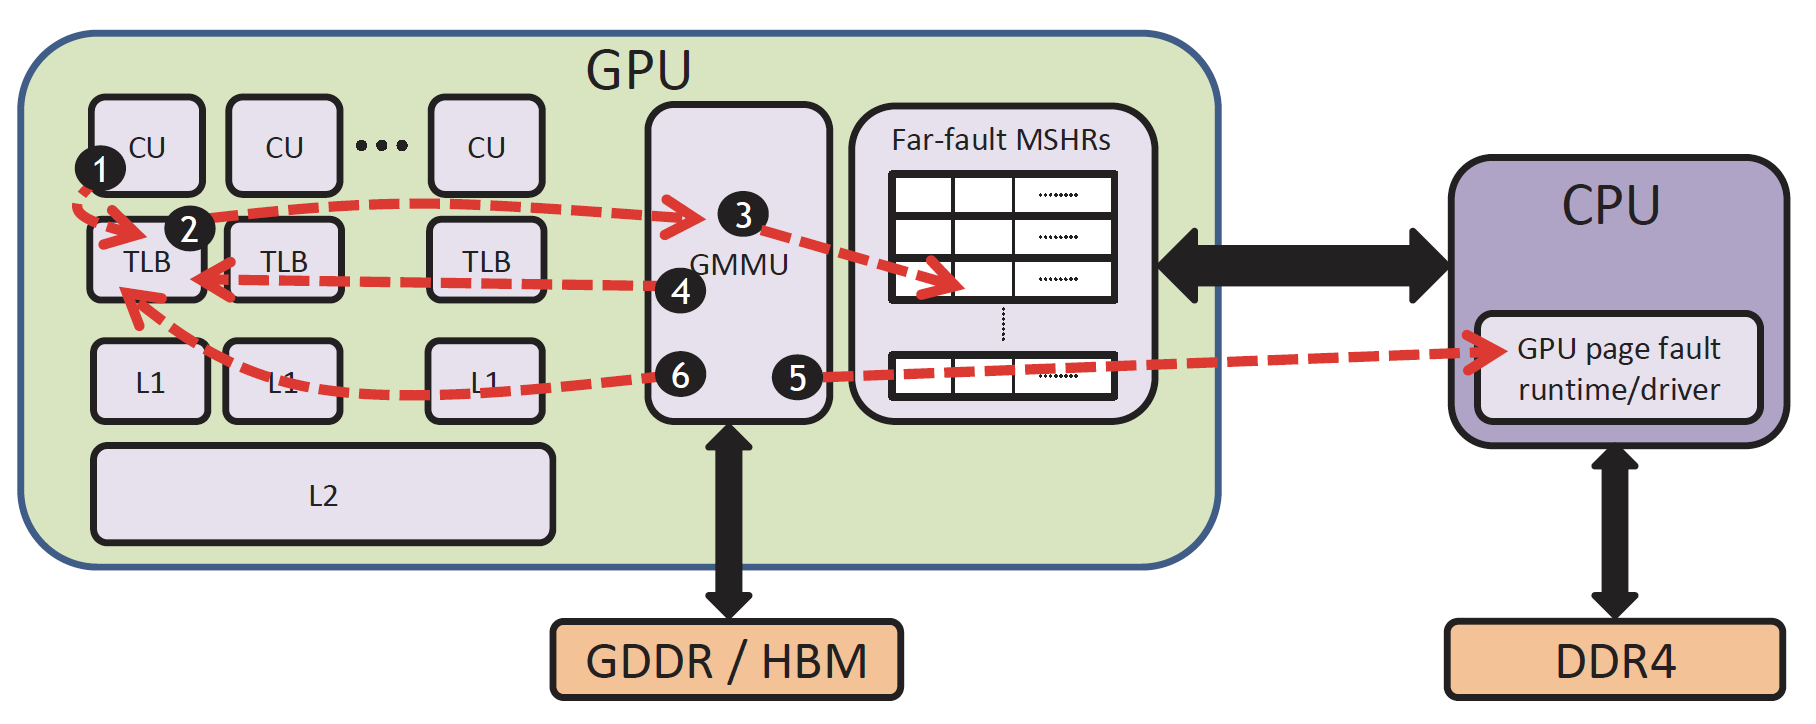
\includegraphics[width=.90\textwidth,keepaspectratio]{figures1/MMU.elf}
      \captionsetup{width=.90\textwidth}
      \caption{Architectural view of GPU MMU and TLBs implementing compute unit (CU) transparent far page faults.
sus}
      \label{fig:mmu}
   \end{figure}